\chapter{Internal Representations in Neural Networks}\label{ch_representations}
\chapterauthor{Jeff Yoshimi}

% More links to linear algebra chapter and similarity spaces and clusters.  In fact, that should perhaps be a separated topic in the linear algebra chapter.
In this chapter we discuss internal representations that develop in neural networks, which is a key theme when considering neural networks in \emph{cognitive science} and ``connectionism'' (see section \extref{connectionism}), which are the emphases in this book. We have seen that  supervised learning methods are not generally take	n to be neurally realistic in their mechanistic details, since there is no obvious way for error to be sent ``backward'' through the dendrite of neurons (section \extref{backprop}).\footnote{However, some circuits have been identified in the brain that may implement error-based supervised learning, \eg climbing fibers in the cerebellum (see chapter \extref{ch_neuro}). Error based learning that is similar in some ways to backprop is also emphasized in predictive coding accounts of the brain and predictive processing accounts of cognition. For a  recent discussion of neural realism of backprop, see \cite{whittington2019theories}.}  However, even if backprop is not realistic, it produces internal representations that are similar to representations humans use.\footnote{That is, even if backprop does not happen in most parts of the brain, it can still be used as a device to discover the kinds of representations that the brain finds. How the brain develops these representations is still a mystery, but backprop let's us at least see what those representations might look like and what function they might serve. The idea that backprop could be used to identify valid neural representations even if it is not biologically realistic was discussed as far back as Zipser's work on system identification, if not earlier. See \cite{zipser1992identification}.}

\section{Internal Representations in Neural Networks}

% It's a bigger deal than that, they _outperform_ similar models in neuroscience

% Glossary entry. See emails to Guatliero. References.
% Does it work as well for motor things?
% Rewrite to get rid of brait repeats
%  More work on "parts" of a representation or state. General picture of space, links to SOM and other chapters
A representation in a neural network is a state (in the sense of ``state'' discussed in \extref{ch_dst},  a pattern of activation over a set of nodes) that reliably occurs in response to some external input. For example, whatever activations occur in a neural network when an apple is present can be thought of as being a representation of apple. Note that a representation can be spread across many nodes, so that we have the input representation and hidden unit representations, for example. They can also have different levels of generality, and this can be unpacked in terms of relations of points in a state space. For example, different apples might all produce slightly different points in state space that are near each other, and different fruits might do the same, etc, producing a nested structure. The details of what a representation are--and whether they are even valuable to posit--are highly contested and controversial, but we simply assume this simple definition here.\footnote{Doubts about representations are associated with embodied cognition, and examples, such as Braitenberg vehicles, which show that one can have intelligent behaviors in a body-world system without there being much value to interpreting internal states. Those who allow representations  often add other components to the definition of a representation. For example, it should be  possible to activate a representation agent state absent its normal cause (representations  are ``detachable'' rather than ``stimulus bound''), which allows for cases of  mis-representation, planning in the absence of the object, and so on. It is generally assumed that  representations are used by the agent to guide its behavior. Many assume that computational processes must transform representations  into other representations, to support adaptive behaviors}
% RSA too?

In this chapter a range of examples of representations are considered, all of which show how, under the pressure of gradient descent, networks trained by backprop and its variants produce psychologically realistic internal representations. Remember this was a theme in the introduction (chapter \extref{ch_intro}). Neural networks are trained, not programmed. They develop useful abilities and, as we will see, internal representations, without having anything programmed in. They develop these abilities and representations simply by learning to perform tasks from data. This was a source of a great deal of excitement in the early ``connectionist'' discussions of the 1980s (section \extref{first_resurgence}). Remember from chapter \extref{ch_applications} that connectionism corresponds to the use of neural networks as cognitive models, which capture psychological and behavioral features of the mind, without concern for neural realism. After the deep learning revolution (section \extref{deep_revolution}), the idea has come back, but with plenty of interest in neural realism as well (computational cognitive neuroscience).  In general, the idea is that neural networks trained by algorithms like backprop are relevant to psychology and neuroscience, \emph{even if backprop itself is not neurally realistic}.
% Rep alignment, etc.

This approach also builds on the visual language we have been developing for understanding the mind, in terms of points or vectors in high dimensional spaces. In section \extref{sect_xor_remap} we saw that multilayer feed-forward networks trained by supervised learning methods (\eg backprop) will re-map an input space in order to make a linearly inseparable problem separable. That was an abstract example, but it also applies to more everyday cases. You should be able to interpret pictures like the one in figure \ref{remappingClusters}.  Points correspond to representations. In this example, black is one category, and white is another. It is similar to the XOR example from section \extref{sect_xor_remap}.  Note that the representations in the input space are not linearly separable (there is no way to draw a line that separates the black from the white dots) but that they are separable in the hidden unit space.
\begin{figure}[h]
\centering
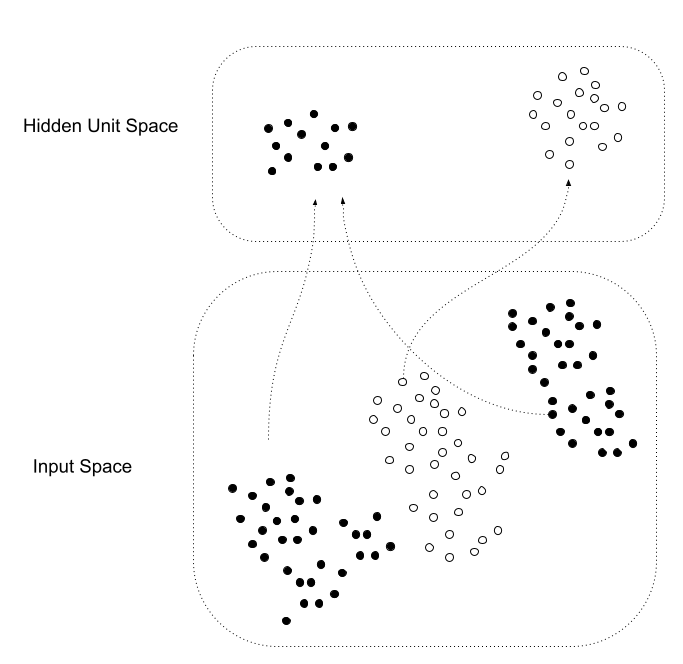
\includegraphics[width=0.5\textwidth]{images/remappingClusters}
\caption[Jeff Yoshimi.]{Remapping a linearly inseparable pair of clusters in the input space to a separable cluster in the hidden unit space. In this graph, colors distinguish different output values associated with states. Each dot corresponds to a a different state, a different representation. Input and hidden unit representations are shown.}
\label{remappingClusters}
\end{figure}

One way to understand how these representations work is that they involve remapping and recombining the input space of a network in various ways. In some cases, as in the one in the figure, separate clusters get merged at another layer.  We also saw this in the the discussion of Selfridge in chapter \extref{ch_history}, how different layers will combine representations of earlier layers to produce complex features. The same idea also comes up in the ``stacked'' layers of a deep network (chapter \extref{ch_cnn}). 
% In other cases, we can imagine that information from context is used to tease apart overlapping clusters, as in  the IRIS case. But this case is more complex, need more input info.

In this chapter a series of examples are given, some of which are elaborations of discussions in other chapters.

% New section. Analytic tools and validation
% See 
% One technique sometimes used to see what internal representations a network has developed is to see what inputs a given node responds to. Gradient descent is used while varying input patterns, with the objective function being neural response. Input space is explored looking for the pattern that most activates a neuron. See the empath example below. Striking examples are also here (that paper, or others at distill.pub, may also have other good information or examples for below).
%Another technique, as in the Elman work, is to show inputs of some class repeatedly, and then take the average activation pattern at a hidden layer.
%There is also this more complex method, which has been used to understand what the neurons in GPT 2 are doing: https://openai.com/research/language-models-can-explain-neurons-in-language-models
% Details on how they are validated
% Validation against responses
% Validation against receptive fields
% Validation by ablation
% Timing: priming, latency effects. Seidenberg and McClelland stuff

\section{Net Talk}

% Add a footnote on this fascinating point: "The distinction between vowels and consonants was  made early; however, the network substituted the same vowel for all vowels and the same consonant for all consonants, which resulted in a babbling sound. A second stage occured when word boundaries are recognized, and the output then resembled pseudowords. After just a few passes through the network many of the words were intelligible, and by 10 passes the text"
NETtalk (1987) \cite{sejnowski1987parallel} was a model of reading English words aloud, created by Terrence Sejnowski and Charles Rosenberg in 1987. The network was trained to speak aloud. The network is a three layer feed-forward network with the structure shown in figure \ref{net_talk}. The input layer codes for a moving window of letters, one of which is taken to be the current input and  the rest of which provide the network with information about neighboring letters.\footnote{Each letter is coded by a 29-dimensional vector (involving one-hot, one-of-29 representations of particular letters, with three additional nodes representing punctuation and word boundaries).} The output layer contains 26 units encoding different features of phonemes including voicing and vowel height. The hidden layer has 80 hidden units. It was presented with written letters in English and was trained to pronounce those letters. There are about 18,000 weights and biases in the network. The network was trained on a corpus of 1000 common words using backprop. It took several days to get the error to a reasonable level using their circa 1987 computer. A slightly modified version of the network could generalize from these 1000 training samples to pronouncing 90 percent of the 20,000 words in a standard English dictionary correctly. The network was shown to perform well with noisy input and to gracefully degrade \cite{sejnowski1987parallel}. 

Here is the key point: the hidden units learned to produce a complete separation of consonants and vowels, even though the network was not told about consonants or vowels. That is, when the central input was a consonant, the hidden unit activation was in one part of the hidden unit space; when it was a vowel it was in another region. Different vowels in the context of different letters produced different points but as a group they were all near each other. Similarly for consonants. The network was not told about the difference between vowels and consonants--it simply learned these categories while it was trained on the pronunciation task \cite{sejnowski1987parallel}. This showed how in learning a mapping from sensory inputs to motor outputs, psychologically meaningful categories could take form in a network's hidden unit space.

\begin{figure}[h]
\centering
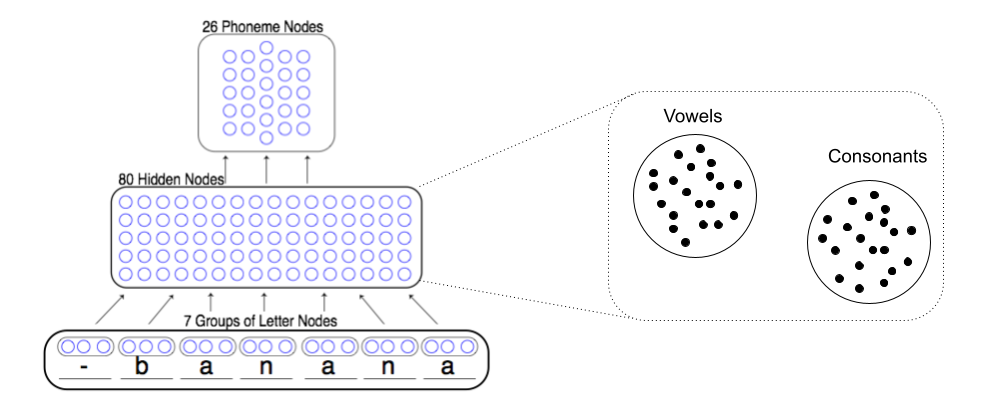
\includegraphics[width=0.8\textwidth]{images/netTalkCategories.png}
\caption[Pamela Payne and Jeff Yoshimi.]{NETtalk models converting written words to sounds, \ie reading aloud. Each letter group has 27 nodes (not the 3 shown). When trained using backprop, it developed internal representations of vowels and consonants, without having been told about them. The idea is schematically shown here. The current central input is an ``n'', a consonant, and so the hidden-unit state would correspond to one of the points in the consonant cluster.}
\label{net_talk}
\end{figure}
% This needs pictures of the vowel vs. consonant part of its state space. That dimension of the discussion is being left out.
% Somehow convey the 27 nodes per group. Maybe just draw them out?  Or use ellipses

One striking feature of this example is that the sounds the networks produced could be artificially synthesized and played back.  I think this had quite an impact on the community at the time, since you could ``hear'' the network learn (listen for yourself at  \url{https://www.youtube.com/watch?v=gakJlr3GecE}). Initially the network produced a babble of sounds, like a baby. But as it came to learn the task it got better and better, until it produced somewhat fluent speech \cite{sejnowski1987parallel}. This made it quite palpable what was going on: the network was slowly getting better, in a way that sounded vaguely like a child learning to read. I encourage you to listen to the (somewhat creepy) process. So again, even if backprop is not neurally plausible, it seems to be doing something \emph{like} what the brain does, and it does so by developing psychologically realistic representations of vowels and constants.
% Expand on the semantic cognition book with a few more paragraphs. It's got very simple and  compelling examples. Maybe also add the development book out of UCSD. 

\section{Elman's Prediction Networks}

%  Mention Simbrain sims.  And see book todos for important notes on how this works.

Another early connectionist analysis of internal representations occurred in the context of Jeff Elman's simple recurrent networks (see chapter \extref{ch_supervised_recurrent}). In a famous paper \cite{elman1990finding}, Jeff Elman trained a simple recurrent network like the one in figure \ref{elman_srn_categories} to predict the next words in a sentence.\footnote{\url{http://psych.colorado.edu/~kimlab/Elman1990.pdf}.}  The input data used to train the network consisted of thousands of sentences generated using a simple ``caveman'' grammar. Some sample sentences generated by this grammar are shown in Fig. \ref{elman_sentences}. The network predicts the next word in  a sentence at any time. For example, it predicts that the word ``cat'' will be followed by ``chase'' or ``eat''. With training, error can be reduced, but it never goes to zero, because a given word can be followed by more than one other word. But some words are more likely than others to follow one another, and so the predictions match these patterns. It also learns some general rules, like expecting verbs after nouns \cite{elman1990finding}.\footnote{Simbrain simulations that partially replicate the results of these papers can be accessed in the script menu as \texttt{elmanPhonemes.bsh} and \texttt{elmanSentences.bsh}.}

\begin{figure}[h]
\centering
\frame{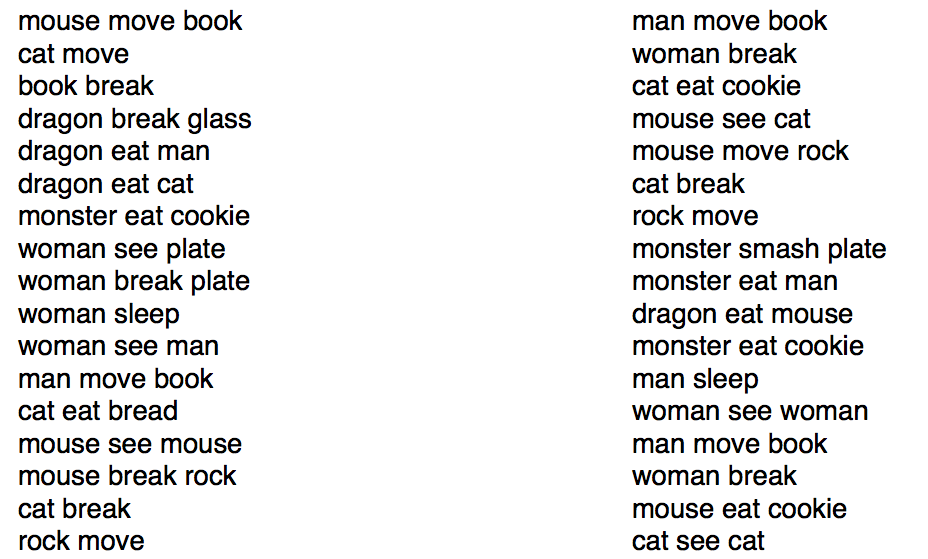
\includegraphics[width=0.65\textwidth]{images/elman_sentences.png}}
\caption[Generated by Jeff Yoshimi based on \cite{elman1990finding}.]{Some of the sentences used to train the word prediction network.}
\label{elman_sentences}
\end{figure}

After being trained to predict the next word in a simple text corpus (the same ``auto-regressive'' approach to training used in transformers like GPT; see chapter \extref{ch_transformers}), the network's internal states were studied. After training, the average response of the network to different words was tested, and it was found that similar words were near each other in the hidden unit space. This can be seen in figure \ref{elman_srn_categories}, which can be thought of as a dimensional reduction of the hidden unit space.\footnote{The original picture this was adapted from was generated by exposing the network to each word in the context of many sentences (\eg ``eat'', ``cat''), and then taking the average hidden unit activation across these exposures. The resulting vectors are like the centers of clusters in the hidden unit space.}  Each point in the right panel of the figure correspond to a vector (an activation pattern) in the hidden unit space, projected to two dimension. Distances between points are meaningful: points closer to each other in the diagram correspond to hidden unit vectors that are closer to each other in the hidden unit space. 

\begin{figure}[h]
\centering
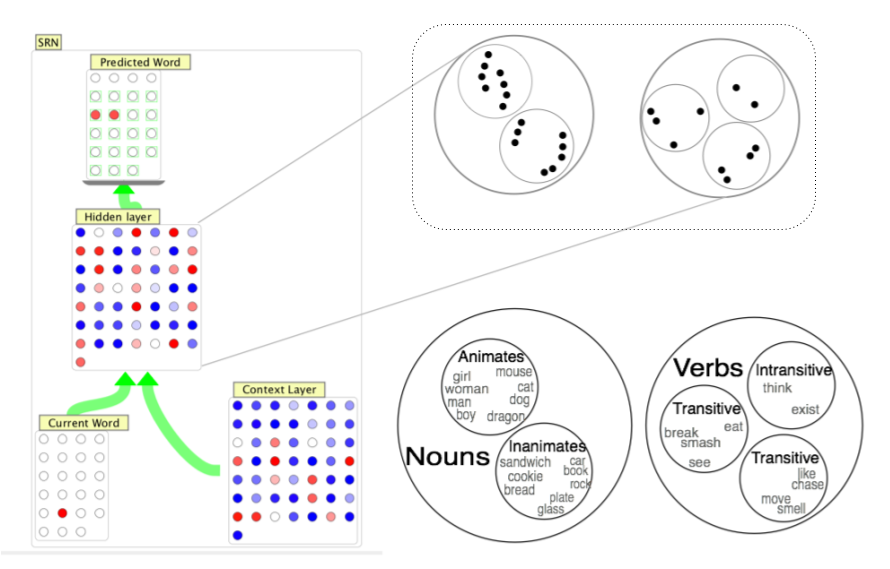
\includegraphics[width=0.8\textwidth]{images/elmanCategoriesSpace.png}
\caption[Jeff Yoshimi.]{The SRN used in the word prediction task. The output layer predicts the next word (coded as a binary vector) in a sentence. It is currently undecided between which of two words might come next. The right top panel shows (schematically, this is not a projection of actual data) what points in the hidden unit space corresponding to different words. The right bottom panel shows how these points cluster in to grammatical and semantic categories. Points in the hidden unit space corresponding to similar words are clustered nearby each other. The image on the bottom-right shows what words the dots correspond to.}
\label{elman_srn_categories}
\end{figure}

Gramatically and semantically similar words are near each other in the hidden unit space and they form into a hierarchical structure. Nouns produce hidden unit representations that are similar to one another and which form into one cluster, and similarly for verbs. Within the nouns we see further clusters for animate vs. inanimate nouns, and there are additional categories as well.\footnote{There are two categories of transitive verbs because some verbs (like ``chase'') are always transitive in the data (that is, taking a direct object), while others (like ``break'') were sometimes transitive, sometimes not.}  The striking thing about this network was that it learned these categories \emph{without being told anything about grammar}. None of the categories apparent in its hidden unit space were directly programmed in to the network: it simply learned them in the process of solving the input-output task it was given (compare the way Nettalk learned phonological categories when learning to read aloud, or the way deep networks develop realistic edge detectors and other feature detectors when trained to recognize objects). 
% Even down to food on one side and glass and late near each other

The network was used to argue against the prevailing view in psycholinguistics, associated with Noam Chomsky, that  grammars are innate, rather than learned.  Elman's work showed that a network with no built-in grammar could acquire the rudiments of a grammar from the environment. Its grammatical categories were not ``built in'' to the network, but learned from the training data--the pattern of words fed to the network.
% Chomsky's response; poverty of stimulus, etc.
% Written quickly; carefully revise and add citations before publication.

\section{Deep Vision Networks}

So far we have focused on cases where we could visualize clusters in a hidden unit space. But there are other ways to show that a network has developed realistic internal representations, which begin to take us from connectionism to computational neuroscience and computational cognitive neuroscience.

% Also V4. Discuss a bit about how V1, V2, V4 different. Cite other papers that discuss other areas.
As discussed in chapter \extref{ch_history}, after the deep learning revolution, neural networks came back in fashion, and scientists once again began turning to these as models of brain and cognition (for example, see  \cite{yamins2014performance, yamins2016using}). Deep networks (chapter \extref{ch_cnn}) trained using backprop to recognize numbers and other objects in images produce activations that match neural responses in such brain areas as V1, V2, and IT, which are discussed in chapter \extref{ch_neuro}.  V1 and V2 are part of early visual processing, with V1 containing edge detectors. IT is part of the ventral stream (also discussed in chapter \extref{ch_neuro}) which is involved in object recognition. The model contains separate layers corresponding to three parts of IT: an anterior, central, and posterior part. The correspondence between layers of the deep net and parts of the brain are shown by green dashed lines in figure \ref{yamins_2016_architecture}.  The similarity of the response of one of the last layers of the deep network and IT neural responses are shown in figure \ref{yamins_2016_responses}.  The model outperforms computational neuroscience models specially designed to model the visual systems of the brain. Simply under the pressure of the gradient descent algorithm, they develop realistic representations. 

% Explain LN is just linear-non-linear which encompasses convolutions, pooling, and dense. pretty much a weight layer and target node layer. DOG is diff of Gaussians and T is transformation and I think the idea is that something of the neuro is understood there, but not in other layers.
\begin{figure}[h]
\centering
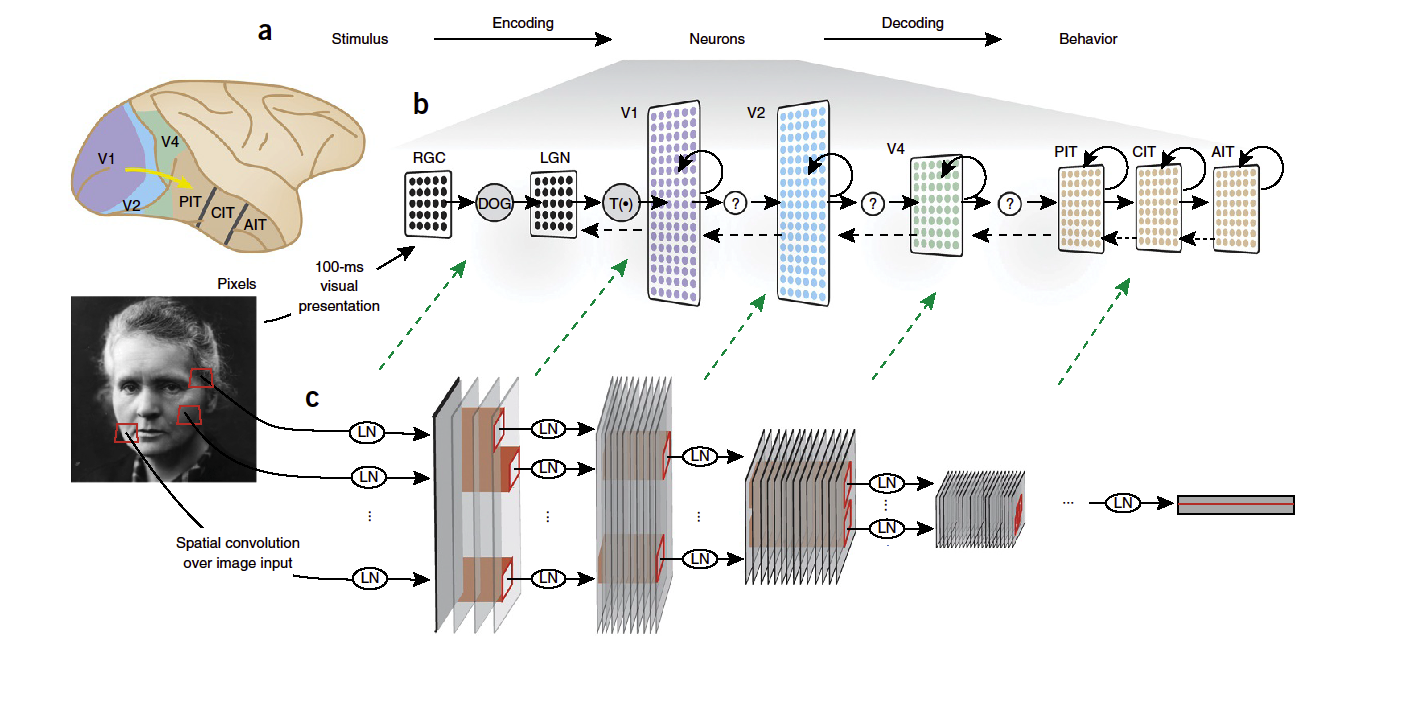
\includegraphics[width=0.8\textwidth]{images/deepNetYaminsArchitecture_2016.png}
\caption[Yamins.]{Architecture of a deep network whose neural responses were compared with neural responses in corresponding regions of the brain. These regions include primary and secondary visual processing areas and several areas of the ventral stream.}
\label{yamins_2016_architecture}
\end{figure}

% Details of which area still not clear, I guess CIT based on green arrow but check note 33 ref
\begin{figure}[h]
\centering
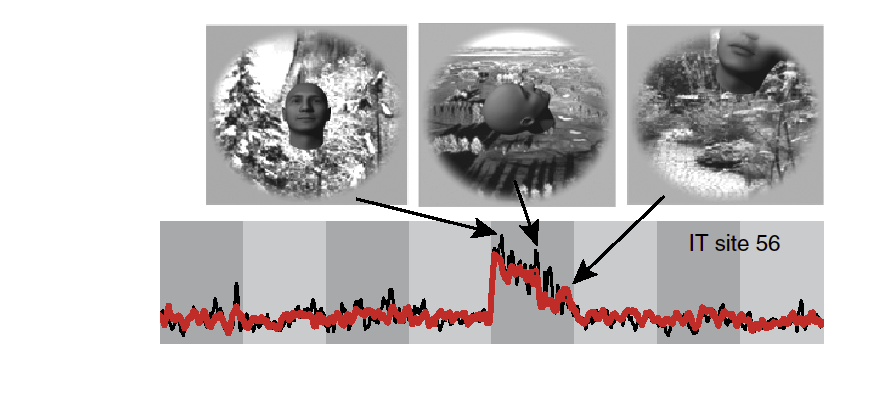
\includegraphics[width=0.6\textwidth]{images/deepNetYaminsITResponses_2016.png}
\caption[Yamins.]{Comparison of node activations in a hidden layer of the deep net (black) shown in figure \ref{yamins_2016_architecture}, with actual neural responses in brain area IT (red). Each point on the x-axis shows how the biological and artificial neural network respond to a particular image. Three sample images are shown above. As can be seen, images with a head in them produce a higher response both in the neural network and in the brain.}
\label{yamins_2016_responses}
\end{figure}

% For a visually striking discussion of these receptive fields, see distill.pub

\section{Other Examples}

There are many other examples of psychologically and neurally realistic internal representations  in artificial neural networks, including examples based on other more realistic learning algorithms. For example, the fixed point attractors of a Hopfield network discussed in chapter \extref{ch_unsupervised_recurrent}, the representations that develop in competitive nets and SOM networks, and psychological elaborations of BERT  (based on the same transformer architecture as GPT) discussed in chapter \extref{ch_transformers}, all have properties that shed light on human cognition. 
% Even  the IAC network discussed in chapter \extref{ch_intro} is realistic in some ways

% OTHER EXAMPLES
% Triangle model
%  \url{https://www.youtube.com/watch?v=gakJlr3GecE}
% Something with action spaces
% Work in Hopfield and Boltzmann cases. Not backprop, but still internal reps
% BERT

% EMPATH
%Gary Cottrell's  (2002) emotion recognition model, EMPATH. ** Developed person detectors with responses similar to IT despite not being told about people.** This network was trained using multiple images of multiple people, each of whom made different facial expressions. The output layer has a one-hot encoding of six basic emotions. Cottrell focused on the second-to-last ``Gestalt'' layer of the network, which  developed nodes that are responsive to particular faces. Like real face-recognition neurons in the ventral stream of cortex (more specifically in area IT), these neurons respond to a picture of someone even if their eyes were occluded, and respond less strongly the more a face image is rotated. The network produced these representations of people even though it was never told about individuals. It was only trained to recognize emotions. It did this entirely on its own, as an artifact of the training process.

%An example is Gary Cottrell's  emotion recognition model, EMPATH, shown in figure \ref{face_net}.\footnote{See \url{http://authors.library.caltech.edu/6983/1/DAIjcn02.pdf} \cite{dailey2002empath}.} This network was trained using multiple images of multiple people, each of whom made different facial expressions. The network had several hidden layers, including a layer of edge detectors (outputs of Gabor filters), and a layer that used principle components analysis or PCA, which is similar to Oja's rule (see chapter \extref{ch_unsupervised}) to do a dimensionality reduction of the previous layer, pulling out the most significant features of that layer. The second-to-last node layer of the network was called a ``Gestalt layer''. It produced responses similar to face-detectors in the ventral stream of the human visual system  (see chapter \extref{ch_neuro}). The output layer has a one-hot encoding of six basic emotions \cite{dailey2002empath}. 
%
%\begin{figure}[h]
%\centering
%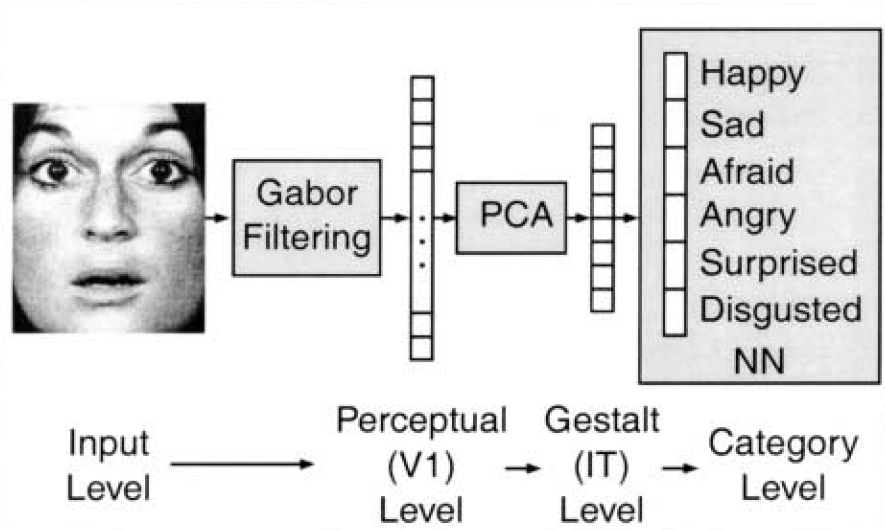
\includegraphics[width=0.5\textwidth]{images/face_network.png}
%\caption[From Adolphs, Cottrell, Dailey and Padgett, 2002  \cite{dailey2002empath}.]{Structure of Cottrell's EMPATH emotion recognition network. On the left is a grid of nodes that respond directly to an image. This layer contains over 40,000 nodes. The image inputs are then processed using a layer of weights (``Gabor filtering'') that produce responses in the ``perceptual level'' nodes similar to responses of edge detector neurons in the visual cortex. Another layer of weights performs PCA to reduce the perceptual level to a ``gestalt'' layer of 50 nodes, that produces responses similar to responses in the ventral steam of the human visual system. The final layer of 6 nodes does the actual classification into different emotion categories, using least mean squares. }
%\label{face_net}
%\end{figure}
%
%Cottrell focused particularly on the second-to-last ``Gestalt'' layer of the network, which  developed nodes that are responsive to particular faces. Cottrell has said that the face recognition nodes in his network act a lot like face recognition neurons in the brain.\footnote{\url{http://tdlc.ucsd.edu/events/boot_camp_2015/Cottrell_Backprop-representations.pdf}.}  Like real face-recognition neurons in the ventral stream of cortex (more specifically in area IT), these neurons respond to a picture of someone even if their eyes were occluded, and respond less strongly the more a face image is rotated. The network produced these representations of people \emph{even though it was never told about individuals}. It was only trained to recognize emotions. It did this entirely on its own, as an artifact of the training process \cite{dailey2002empath}. 
%
%% Finding optimal stimulator for an internal node using gradient descent (in a new way).
%One thing you can do with this kind of network is visualize the internal representations it develops. If you focus on one of the face recognition nodes, and then find what visual input it is most tuned to, a ``ghostly looking face'' can be observed (see figure \ref{holon}). This image is a kind of visualization of the network's internal template or representation for a particular person \cite{dailey2002empath}. It might be similar to what gets activated in dreams and imagination.\footnote{For a more recent example that takes this idea much further, see \url{https://research.googleblog.com/2015/06/inceptionism-going-deeper-into-neural.html} \cite{mordvintsev2015inceptionism}. Also see \url{https://distill.pub/2017/feature-visualization/}.}
%% https://en.wikipedia.org/wiki/Eigenface
%% Need proper citation for distill article
%% The resulting low-dimensional object-level representation is specific to the facial expression and identity variations in its input, as is the population of so-called face cells in the inferior temporal cortex
%% any face in training set a linear combination of eigenfaces. 
%% especially clear in https://www.cs.ucsb.edu/~mturk/Papers/jcn.pdf
%
%\begin{figure}[h]
%\centering
%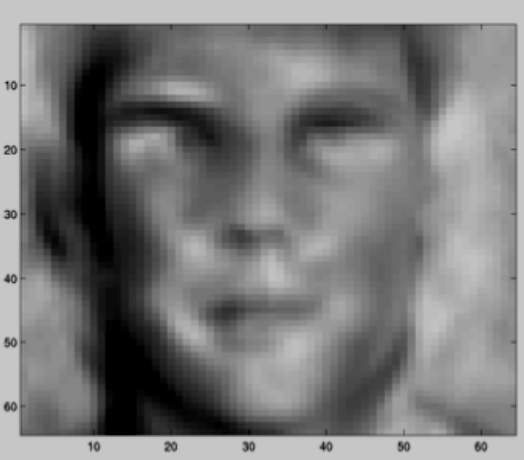
\includegraphics[width=0.3\textwidth]{images/holon.png}
%\caption[From \url{http://cseweb.ucsd.edu/\~gary/258a/Backprop.pdf}.]{Optimal input pattern for a hidden (``Gestalt'') layer face node. Shows what kinds of inputs the unit will respond to.}
%\label{holon}
%\end{figure}
%

% Things to work on with EMPATH
% Clarify which part is backprop. Not clear now in pics
% Does not follow nicely on xor the way nettalk does, in that the hidden layer reps are not as obviously psychologically relevant. Either improve description of them or change order.
% Relatedly, why do we care here about individual faces? In a way it's an artifact, isn't it?  In fact. since 14*6 = 84, it seems it might have just learned to distinguish happy, said, etc. for each person, then map from those to the output layer. I guess that's ok. But an individual face is not really an eigenface, so I'm missing something.
% Explain how this sets up  deep nets, which also both find features on their own (convolutional layers) and then compress via downsampling
% It is notable that the data is based on Ekman's famous work on facial expressions. Add that, at least in a footnote. Citation to POFA database (see Figure 1a) (Ekman & Friesen, 1976). \cite{ekman1976pictures} Note Ekman, also at UCSD, is a famous psychoogist who used this dataset used to argue for universality of basic emotions. "Through a series of studies, Ekman found a high agreement across members of diverse Western and Eastern literate cultures on selecting emotional labels that fit facial expressions. Expressions he found to be universal included those indicating wrath, grossness, fear, joy, loneliness, and shock", "This data set contains photos of 14 actors portraying expressions that are reliably classified as happy, sad, afraid, angry, surprised, or disgusted by naive observers"


% HINTON BACKPROP
% In another example, due to Hinton, backprop was used to train a network to describe relationships between members of two families, one American and one Italian. The network could be asked a question like ``who was Sophia's sister". The network developed hidden layer nodes that  represented whether a given person was Italian or American, and whether a person was first-generation, second-generation, etc. Using this information the network could draw inferences. What is interesting is that it developed these representations of nationality and generation without being told to \cite{hinton1986learning}.

